% Created 2018-11-26 月 09:40
% Intended LaTeX compiler: pdflatex
\documentclass[presentation,dvipdfmx,CJKbookmarks]{beamer}
\usepackage{CJKutf8}
\usepackage{atbegshi}
\AtBeginShipoutFirst{\special{pdf:tounicode UTF8-UTF16}} % for UTF-8
\usepackage[utf8]{inputenc}
\usepackage[T1]{fontenc}
\usepackage{graphicx}
\usepackage[export]{adjustbox}
\usepackage{lmodern}
\usepackage{grffile}
\usepackage{longtable}
\usepackage{wrapfig}
\usepackage{rotating}
\usepackage[normalem]{ulem}
\usepackage{amsmath}
\usepackage{textcomp}
\usepackage{amssymb}
\usepackage{capt-of}
\usepackage{hyperref}
 \usepackage{minted}
\usetheme{default}
\usecolortheme{lily}
\author{包昊军(钧钩)}
\date{2014-01-20}
\title{Android网络和数据}
\hypersetup{
 pdfauthor={包昊军(钧钩)},
 pdftitle={Android网络和数据},
 pdfkeywords={},
 pdfsubject={},
 pdfcreator={Emacs 26.1 (Org mode 9.1.9)}, 
 pdflang={English}}
\begin{document}
\begin{CJK*}{UTF8}{simsun}

\maketitle
\begin{frame}{Outline}
\tableofcontents
\end{frame}

\CJKtilde

\begin{enumerate}
\item 回顾
\label{sec:org5aae1b3}

\begin{frame}[label={sec:org939d671}]{上节内容}
\begin{block}{ListView \& Adapter}
\end{block}
\begin{block}{实现banner和列表视图List的同时滑动}
\end{block}
\begin{block}{删除列表中一行}
\end{block}
\begin{block}{双列列表}
\end{block}
\end{frame}

\begin{frame}[label={sec:org3cb7c42}]{往期回顾}
\begin{block}{Android系统和环境}
\end{block}
\begin{block}{Activity等四大组件}
\end{block}
\begin{block}{ListView}
\end{block}
\end{frame}
\item 工具
\label{sec:org14d2916}
\begin{frame}[label={sec:org87b6b9c}]{粗野的Beagrep}
\begin{block}{Grep 9G Android代码,只需0.23秒}
\end{block}
\begin{block}{阅读源代码的利器之一}
\end{block}
\end{frame}
\begin{frame}[label={sec:org8f0836b}]{精细的grep-gtags}
\begin{block}{综合了ctags (exuberant)、gtags、cscope}
\end{block}
\begin{block}{可以与beagrep组合使用,获取函数调用位置}
\end{block}
\begin{block}{可以定位png文件,xml元素,这些也是源代码:-)}
\end{block}
\end{frame}
\begin{frame}[label={sec:org0a671af}]{搞笑的Ajoke}
\begin{block}{主要在使用grep-gtags和一些自制脚本}
\end{block}
\begin{block}{可以打印继承树}
\begin{itemize}
\item 目前不可以打印倒继承树
\end{itemize}
\end{block}
\begin{block}{可以补齐函数}
\end{block}
\begin{block}{可以自动import}
\end{block}
\begin{block}{可以重载函数}
\end{block}
\begin{block}{将来会支持Exception}
\end{block}
\end{frame}
\begin{frame}[label={sec:org3764a63}]{可怕的skeleton-complete.el}
\begin{block}{打几个字符(骨架),补全整字、整句、整行、整段(血肉)}
\end{block}
\begin{block}{其实firefox也有类似的功能}
\end{block}
\begin{block}{Java IDE神器 IntelliJ IDEA 也有类似的功能}
\end{block}
\end{frame}

\begin{frame}[label={sec:org3ecba9c}]{yasnippet}
\begin{block}{另一个非常强大的补齐展开工具}
\end{block}
\begin{block}{用起来更正式,需要提前准备好展开脚本}
\end{block}
\end{frame}

\item 网络
\label{sec:orgc581fe0}
\begin{frame}[label={sec:org69d0895}]{网络编程介绍}
\begin{block}{Socket(套接字)}
\begin{itemize}
\item Tcp,Udp,Unix Domain
\item 我的输入法编程
\end{itemize}
\end{block}

\begin{block}{HTTP通讯}
\begin{itemize}
\item HttpURLConnection (Android原生,性能更好)
\item DefaultHttpClient (apache代码,早期bug较少)
\end{itemize}
\end{block}

\begin{block}{WebView}
\begin{itemize}
\item 频繁变化,或轻交互
\end{itemize}
\end{block}
\end{frame}


\begin{frame}[label={sec:orgfdcf4c1}]{小练习}
\begin{block}{获取一段JSON数据 (MainActivity1)}
\begin{itemize}
\item AllIn4Demo代码位置
\url{http://10.125.206.165/allin4.zip}
\end{itemize}
\end{block}
\begin{block}<2->{会出错}
\end{block}
\end{frame}
\begin{frame}[label={sec:orgb5780b6}]{UI主线程和联网线程}
\begin{block}{Android编程中,需要牢记:}
\begin{itemize}
\item 要区分开UI主线程和工作线程
\end{itemize}
\end{block}

\begin{columns}
\begin{column}{0.4\columnwidth}
\begin{block}{Android网络操作必须用工作线程}
\end{block}
\end{column}
\begin{column}{0.4\columnwidth}
\begin{block}<2->{会阻塞,导致无响应}
\end{block}
\end{column}
\end{columns}
\begin{columns}
\begin{column}{0.4\columnwidth}
\begin{block}{工作线程不允许操作UI元素}
\end{block}
\end{column}
\begin{column}{0.4\columnwidth}
\begin{block}<3->{操作UI元素的API都是线程不安全的,只能在一个线程中调用以保证线程安全}
\end{block}
\end{column}
\end{columns}
\end{frame}

\begin{frame}[label={sec:orgbd63715}]{工作线程与UI主线程间通信}
\begin{block}{runOnUiThread}
\begin{itemize}
\item 工作线程中调用操作UI元素的Callback函数
\end{itemize}
\end{block}
\begin{block}{Handler}
\begin{itemize}
\item 工作线程发送消息,UI线程处理消息
\item 当然UI线程也可以给自己发消息
\end{itemize}
\end{block}

\begin{block}{AsyncTask}
\begin{itemize}
\item 更好的封装,有准备、运行(进度)、结果三个阶段
\end{itemize}
\end{block}
\end{frame}

\begin{frame}[fragile,label={sec:orgb30629a}]{runOnUiThread}
 \begin{minted}[]{java}
// In UI thread:
new Thread(new Runnable() {
   @Override
   public void run() {
     // do some work in working thread
     runOnUiThread(new Runnable() {
       @Override
       public void run() {
         // manipulate the UI elements
         // within runOnUiThread
         mTextView.setText(mGetJsonHelper.result);
       }
     });
   }
}).start();
\end{minted}
\end{frame}

\begin{frame}[fragile,label={sec:orgfeef6a4}]{Handler}
 \begin{minted}[]{java}
Handler mHandler = new Handler() {
  public void handleMessage(Message msg) {
    switch (msg.what) { ... }
    super.handleMessage(msg);
  }
};
new Thread(new Runnable() {
   public void run() {
     // do something in working thread
     Message message = new Message();
     message.what = 1;
     message.setData(Bundle b);
     mHandler.sendMessage(message);
   }
}).start();
\end{minted}
\end{frame}

\begin{frame}[fragile,label={sec:org96ee0b3}]{AsyncTask}
 \begin{minted}[]{java}
private class MyAsyncTask
 extends AsyncTask<Param, Progress, Result> {
  protected void onPreExecute()
  {...}
  protected Result doInBackground(Param... args)
  { publishProgress(...); return ""; }
  protected void onProgressUpdate(Progress... args)
  {...}
  protected void onPostExecute(Result parsedText) {
    mTitleBar.startAnimation(mSlideOut);
  }
}
new MyAsyncTask().execute(...);
\end{minted}
\end{frame}
\begin{frame}[label={sec:org6f9e31d}]{小练习}
\begin{block}{用 runOnUiThread 实现线程间交互 (MainActivity2)}
\end{block}
\begin{block}{用 Handler 实现线程间交互 (MainActivity3)}
\end{block}
\begin{block}{用 AsyncTask 实现线程间交互 (MainActivity4)}
\end{block}
\end{frame}

\begin{frame}[label={sec:org4427f39}]{WebView应用}
\begin{block}{微博、微信客户端等的网页(网络应用)}
\end{block}
\begin{block}{CrossDict的实现(离线网页应用)}
\end{block}
\end{frame}

\item 数据
\label{sec:org678f738}
\begin{frame}[label={sec:org769e8a7}]{Android文件系统介绍}
\begin{block}{ADB的使用}
\end{block}
\begin{block}{Android文件系统目录结构}
\end{block}
\begin{block}{App目录结构}
\end{block}
\end{frame}

\begin{frame}[label={sec:org3757fe6}]{小练习}
\begin{itemize}
\item 用ADB安装Apk
\item 用ADB卸载Apk
\item 查看App的目录
\end{itemize}
\end{frame}

\begin{frame}[fragile,label={sec:org1602a59}]{Android系统数据存取}
 \begin{block}{SharedPreferences}
\begin{minted}[]{java}
SharedPreferences spf =
  getSharedPreferences("allin4", 0);
spf.getInt(String key, int defValue);
spf.edit().putFloat(String key, float value).commit();
\end{minted}
\end{block}

\begin{block}{File:私有文件,sdcard上的文件,只读的asset资源文件}
\begin{minted}[]{java}
openFileInput(path); openFileOutput(path);
Environment.getExternalStoragePublicDirectory(path);
AssetManager am = getAssets(); am.open(path);
\end{minted}
\end{block}
\begin{block}{Sqlite 单进程}
\end{block}
\begin{block}{ContentProvider 多进程(联系人数据)}
\end{block}
\end{frame}
\begin{frame}[label={sec:orgf6a757f}]{小练习}
\begin{block}{SharedPreferences}
\begin{itemize}
\item 每进一次Activity,把记数加1,并显示
\item 查看 SharedPreferences 在文件系统中保存的位置
\end{itemize}
\end{block}
\end{frame}

\begin{frame}[fragile,label={sec:org85247b5}]{数据传递、共享}
 \begin{block}{Intent传递数据}
\begin{minted}[]{java}
Intent intent = new Intent();
intent.setClass(thisActivity,
  thatActivity.class);
intent.putExtra(key, value);
startActivity(intent);
\end{minted}
\end{block}

\begin{block}{Intent获取数据}
\begin{minted}[]{java}
Intent intent = getIntent();
value = intent.getStringExtra(key);
\end{minted}
\end{block}
\end{frame}
\begin{frame}[fragile,label={sec:orgc8b4406}]{数据传递、共享(续)}
 \begin{block}{startActivityForResult}
\begin{minted}[]{java}
Intent intent = new Intent(thisActivity,
       thatActivity.class);
startActivityForResult(intent, GET_CODE);

setResult(RESULT_OK,
    (new Intent()).setAction("Corky!"));
\end{minted}
\end{block}
\begin{block}{onActivityResult}
\begin{minted}[]{java}
protected void onActivityResult(
 int requestCode,
 int resultCode,
 Intent data) {
  if (requestCode == GET_CODE) {...}
}
\end{minted}
\end{block}
\end{frame}
\begin{frame}[label={sec:org852b592}]{数据传递、共享(续)}
\begin{block}{Singleton、Application}
\end{block}
\begin{block}{数据存取也是一种IPC}
\end{block}
\end{frame}

\begin{frame}[label={sec:org7b29113}]{小练习}
\begin{itemize}
\item 用Intent传递数据
\item 用startActivityForResult获取结果
\end{itemize}
\end{frame}

\item 总结
\label{sec:org1fc3930}
\begin{frame}[label={sec:org9596c90}]{查看文档的方法}
\begin{block}{bhj-help-java 查看java API}
\end{block}
\begin{block}{bhj-help-it 查看android:layout\(_{\text{toLeftOf}}\) android:layout\(_{\text{weight}}\)}
\end{block}
\begin{block}{上beagrep暴力搜索}
\end{block}
\end{frame}
\begin{frame}[fragile,label={sec:orgb7c590a}]{下载整个Android源代码}
 \begin{minted}[]{sh}
repo_url=$(
    echo -n https://github.com/baohaojun
    echo -n system-config/raw/master/bin/repo
)
wget $repo_url -o ~/system-config/bin/repo

mani_url=$(
    echo -n https://android.googlesource.com/
    echo -n platform/manifest
)
repo init -u $mani_url -b android-4.4_r1
repo sync
\end{minted}
\end{frame}
\begin{frame}[label={sec:orga75515f}]{ApiDemos}
\begin{figure}[htbp]
\centering
\includegraphics[width=.5\linewidth]{./images/opengl.ps}
\caption{\label{fig:org9b0feae}
OpenGL画图}
\end{figure}
\end{frame}

\begin{frame}[label={sec:org86ab5b7}]{多读,多写!}
\begin{block}{写出有趣的软件,发布到Google Play上}
\end{block}
\end{frame}
\end{enumerate}
\end{CJK*}
\end{document}
